\documentclass[12pt]{article}
\usepackage{xeCJK}
\setCJKmainfont[]{Noto Serif CJK TC}
\usepackage[top=2cm, bottom=2cm, left=3cm, right=3cm]{geometry}
\usepackage{setspace}
\onehalfspacing
\usepackage{xcolor}
\usepackage{graphicx}
\usepackage{fancyhdr}
\pagestyle{fancy}
\lhead{二分搜尋法}
\usepackage{graphicx}

% code
\usepackage{listings}
\usepackage{color}

\definecolor{dkgreen}{rgb}{0,0.6,0}
\definecolor{gray}{rgb}{0.5,0.5,0.5}
\definecolor{mauve}{rgb}{0.58,0,0.82}

\lstset{frame=tb,
  language=C++,
  aboveskip=3mm,
  belowskip=3mm,
  showstringspaces=false,
  columns=flexible,
  basicstyle={\small\ttfamily},
  numbers=none,
  numberstyle=\tiny\color{gray},
  keywordstyle=\color{blue},
  commentstyle=\color{dkgreen},
  stringstyle=\color{mauve},
  breaklines=true,
  breakatwhitespace=true,
  tabsize=3
}
% code

\begin{document}
    \section{重點整理}
    \subsection{注意事項}
    \begin{itemize}
        \itemsep=5pt
        \item 要二分搜的東西必須是具備\textbf{單調性}
        \item 單純的二分搜:$\log{n}$的測資範圍可以到$10^{18}$,$n\log{n}$則可以到$5\times10^5$
        \item \textbf{範圍的初始左右界設定錯誤}
        \item 取$mid$的時候發生溢位
        \item 最後的$mid$不一定是答案
        \item 負數範圍上二分搜使用錯誤寫法
    \end{itemize}

    \subsection{使用時機}
    \begin{itemize}
        \item 尋找元素
        \item \textbf{二分搜答案}
        \item 最小化最大值/最大化最小值
        \item 第k大/小問題
    \end{itemize}

    \subsection{二分搜工具}
    \lstinputlisting{resource/binary_search_tool.cpp}
    \pagebreak

    \subsection{二分搜模板}
    \lstinputlisting{resource/binary_search_template.cpp}
    \pagebreak

    \section{二分搜簡介}
    \subsection{概念}
    二分搜尋法(簡稱二分搜)的概念非常簡單,就如同遊戲「終極密碼」一樣,請參考以下範例\\
    
    \begin{figure}[h]
        \centering
        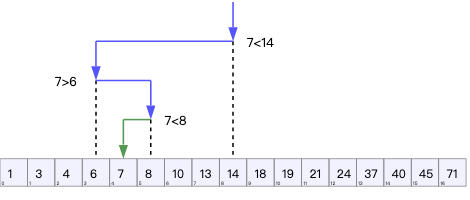
\includegraphics{resource/binary_search_example.png}
    \end{figure}

    \noindent
    以上為最佳的遊玩策略,每次都選擇所有可能的數字的中位數\\
    這就是二分搜的概念,此外,我們可以保證在此情況按照此策略可以在4次猜測以內找到答案,套用在程式的概念,就是可以保證時間複雜度是好的\\\\
    \noindent\textbf{總結:二分搜是一種搜尋技巧,可以在找到是否有一個值(以及他的位置)}

    \subsection{複雜度分析}
    由於上面的概念很簡單,我們可以先做簡單的複雜度分析\\
    由於每次都會減少一半的數值,直到只剩下一個可能的值,我們可以以此逆推\\\\

    設元素的總數量為$n$,每次都會減少一半的元素,可知每次查詢的時間複雜度為$\log_2{n}$可用$O(\log{n})$表示\\
    可處理的上限的範圍可到$10^{18}$,是個非常快速的搜尋法
    \pagebreak

    \section{0/1二分搜}
    接下來是非常間單且經典的問題,會給予一個長度為$n$的陣列,並且陣列的前段皆為連續的0,後段皆為連續的1,目標是要尋找最左邊的1
    \lstinputlisting{resource/01_binary_search_example.txt}

    \noindent
    以上的例題實際上與前述的「終極密碼」非常相似,我們可以使用相同的規則,但是如果得到的值為0,就當作數值太小,否則當作數值太大
    

\end{document}